\documentclass[12pt]{report}

\usepackage{amsmath,amssymb,amsthm,bm,caption,float,geometry,mathrsfs,titlesec}
\usepackage{tikz,tkz-euclide,wrapfig}

\usepackage[math]{cellspace}
\geometry{a4paper, margin=1in}

\title{Projective Geometry}
\author{Saroj Kumar \and Supervisor: Dr. Steven Spallone}
\date{}

\titleformat{\chapter}
    [frame]
    {\bfseries\Huge}
    {\Large CHAPTER \thechapter}
    {1ex}{\centering}[]

\DeclareCaptionFormat{capfmt}{\textbf{#1 #2}#3}
\captionsetup{format=capfmt}

\newtheorem{theorem}{Theorem}
\newtheorem{definition}{Definition}
\newtheorem*{notation}{Notation}

\newcommand\conop{\oplus_{\vphantom{\dfrac{}{}}O}}
\newcommand\tgrp[3]{\mathrm{#1}_{#2}(\mathbb{#3})}
\newcommand\SO[2]{\tgrp{SO}{#1}{#2}}
\newcommand\AffF[2]{\mathbb{A}^{#1}(\mathbb{#2})}
\newcommand\Aff[1]{\mathbb{A}^{#1}}
\renewcommand\qedsymbol{$\blacksquare$}

\DeclareMathOperator{\A}{A}
\DeclareMathOperator{\GA}{GA}
\DeclareMathOperator{\GL}{GL}
\DeclareMathOperator{\Hom}{Hom}
\DeclareMathOperator{\End}{End}

\setlength{\cellspacetoplimit}{5pt}
\setlength{\cellspacebottomlimit}{5pt}

\begin{document}

\begin{titlepage}
    \centering
    \fbox{
        \begin{minipage}[t][0.96\textheight][t]{0.96\textwidth}
            \begin{center}
                \vfill

                \textbf{\Huge PROJECTIVE GEOMETRY} \\

                \vspace{5ex}

                {\Large Saroj Kumar} \\

                \vspace{1ex}

                {\large 20231224}

                \vfill

                {\large supervised by} \\

                \vspace*{1ex}

                {\Large Dr. Steven Spallone} \\

                \vspace{0.1\textheight}

                {Summer 2025} \\

                \vspace{0.1\textheight}
            \end{center}
        \end{minipage}
    }
\end{titlepage}

\tableofcontents{

\chapter{Conics} \label{ch:conics}

The majority of this chapter is based on the ideas presented in Shirali's article
on conic groups \cite{shirali}. We'll also develop this further with the chapter
on conics over characteristic two fields.

\section{Group Laws on Conics}

Consider a non-degenerate conic section $\mathcal{C}$ and a point $O \in
\mathcal{C}$. For any points $P,Q\in\mathcal{C}$, let $\ell'$ be the line passing
through $O$ such that $\ell' \parallel \ell$ where $\ell$ is the line joining $P$
and $Q$. If $\ell'$ intersects $\mathcal{C}$ at a point other than $O$, call that
point $R$. Otherwise, take $R=O$. Define a binary operation
$\conop : \mathcal{C} \times \mathcal{C} \to \mathcal{C}$ as $P \conop Q := R$.
\vspace{1ex}

\begin{figure}[H]
    \center
    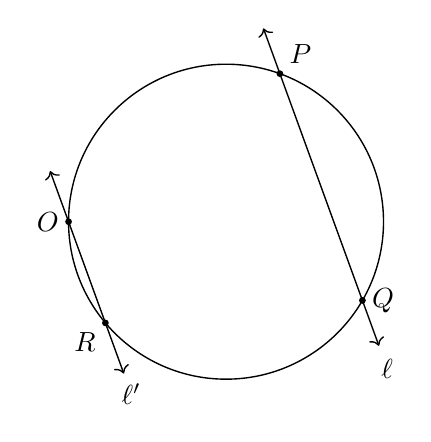
\begin{tikzpicture}
        \tkzDefPoint(0,0){C}
        \tkzDefPoint(-2,0){O}
        \tkzDefPoint({2*cos(70*pi/180)},{2*sin(70*pi/180)}){P}
        \tkzDefPoint({2*cos(-30*pi/180)},{2*sin(-30*pi/180)}){Q}
        \tkzDefPoint({2*cos(-140*pi/180)},{2*sin(-140*pi/180)}){R}

        \tkzDrawPoints[fill=black](O,P,Q,R)
        \tkzDrawLine[<->,line width=0.5,add=0.2 and 0.2](P,Q)
        \tkzDrawLine[<->,line width=0.5,add=0.5 and 0.5](O,R)
        \tkzDrawCircle[color=black,line width=0.5](C,O)

        \tkzLabelPoints[left](O)
        \tkzLabelPoints[above right](P)
        \tkzLabelPoints[right](Q)
        \tkzLabelPoints[below left](R)

        \tkzLabelLine[pos=1.3](P,Q){$\ell$}
        \tkzLabelLine[pos=1.7](O,R){$\ell'$}
    \end{tikzpicture}

    \caption{$P \conop Q$ when $\mathcal{C}$ is a circle.}
\end{figure}

We'll first find formulae to calculate $P \conop Q$ and then proceed to prove
that $\mathcal{C}$ is a group with $\conop$.
\subsection*{A Note on Standard Forms}

Throughout this section, we'll only use standard forms of non-degenerate conics
i.e. circle, rectangular hyperbola and parabola with equations $x^2+y^2=1$, $xy=1$
and $y=x^2$ respectively. In the next chapter, we'll show that any ellipse,
hyperbola and parabola is affine-congruent to these standard forms; generalizing
our results to all conics.

\subsection*{Circle}

If $\mathcal{C}=\mathcal{S}$ with equation $x^2+y^2=1$, any point
$P\in\mathcal{S}$ has coordinates $(\cos t,\sin t)$ where $t\in[0,2\pi)$ is the
angle $P$ forms with the positive $x$-axis in the counter-clockwise direction.
\vspace{1ex}

Let $O,P,Q,R\in\mathcal{P}$ be points with parameters $t_0$, $t_1$, $t_2$ and
$t_3$ respectively such that $P \conop Q = R$. By definition of $P \conop Q$, we
have $PQ \parallel OR$. Note that if $P=Q$, then slope at $P$ is
\[
    y'|_{x=t_1} = \left(-\frac{x}{y}\right)_{t=t_1}
    = \left(-\frac{\cos t}{\sin t}\right)_{t=t_1}
                = -\cot t_1
                = -\cot \left(\frac{t_1+t_2}{2}\right)
\]
and if $P \neq Q$, then $t_1 \neq t_2$ and slope of $PQ$ is 
\[
    \frac{\sin t_2 - \sin t_1}{\cos t_2 - \cos t_1}
    = -\frac{\sin\left(\frac{t_2-t_1}{2}\right)\cos\left(\frac{t_2+t_1}{2}\right)}{\sin\left(\frac{t_2-t_1}{2}\right)\sin\left(\frac{t_2+t_1}{2}\right)}
    = -\cot\left(\frac{t_2+t_1}{2}\right)
\]
Also note that $\sin\left(\frac{t_2 - t_1}{2}\right)$ can be cancelled as it's
only zero when $t_2=t_1+2n\pi$ which means $P=Q$. So, we don't need to consider
the points being same as a separate case. Equating slopes of $PQ$ and $OR$, we
get,
\begin{align*}
    &-\cot\left(\frac{t_2+t_1}{2}\right) = -\cot\left(\frac{t_3+t_0}{2}\right) \\
    \implies& \frac{t_2+t_1}{2} = n\pi+\frac{t_3+t_0}{2} \\
    \implies& t_3 = t_2 + t_1 - t_0 - 2n\pi
\end{align*}

\noindent
As shifts of $2n\pi$ don't affect $t_3$, we can ignore that term on the RHS.
Thus for any $P,Q\in\mathcal{S}$ with parameters $t_1$ and $t_2$
respectively for circle $\mathcal{S}$, $P \conop Q = R$ has parameter
$t_3 = t_1 + t_2 - t_0$ where $t_0$ is the parameter for point
$O$. Note that we always add or subtract multiples of $2\pi$ to make sure
$t_3\in[0,2\pi)$.
\vspace{1ex}

It is easy to see that $\conop$ satisfies closure for $\mathcal{S}$. We'll verfiy each of 
the group axioms now.

\begin{enumerate}
    \item{\textbf{Identity:}} For any $P \in \mathcal{S}$ with parameter $t$,
        $P \conop O$ will have parameter
        \[ t' = t + t_0 - t_0 = t \]
        Thus $O$ acts as the identity element for $\conop$.

    \item{\textbf{Inverse:}} The point $Q\in\mathcal{S}$ with parameter
        $2t_0 - t$ gives the parameter of $P \conop Q$ to be
        \[ t' = t + 2t_0 - t - t_0 = t_0 \]
        Hence, $Q$ is the inverse of $P$.

    \item{\textbf{Associativity:}} For any $P,Q,R \in \mathcal{S}$ with parameters\
        $t_1$, $t_2$ and $t_3$ respectively, $P\conop(Q \conop R)$
        has parameter
        \[
            t_1 + (t_2 + t_3 - t_0) - t_0 =
            t_1 + t_2 + t_3 - 2t_0
        \]
        On the other hand, $(P \conop Q)\conop R$ has parameter
        \[
            (t_1 + t_2 - t_0) + t_3 - t_0 =
            t_1 + t_2 + t_3 - 2t_0
        \]
        Thus $\conop$ is associative.
\end{enumerate}

\noindent
This shows that $\mathcal{S}$ is a group with $\conop$.

\begin{theorem}
    $\langle \mathcal{S},\conop \rangle \cong \langle S^1,\cdot \rangle$ where
    $S^1=\{e^{i\theta}\in\mathbb{C}: \theta \in [0,2\pi)\}$.
\end{theorem}

\begin{proof}
    Consider $\varphi:\mathcal{S} \to S^1$ given by
    $\varphi((\cos\theta,\sin\theta)) = e^{i(\theta-\theta_0)}$. For any points
    $P,Q\in\mathcal{S}$ parametrized by $\theta_1$ and $\theta_2$ respectively,
    $P \conop Q$ has parameter $\theta_1 + \theta_2 - \theta_0$. So,
    \[
        \varphi(P \conop Q) = e^{i(\theta_1 + \theta_2 - 2\theta_0)}
        = e^{i(\theta_1 - \theta_0)}e^{i(\theta_2 - \theta_0)} = \varphi(P)\varphi(Q)
    \]
    Thus $\varphi$ is a homomorphism.
    \vspace{1ex}

    \noindent
    If $\varphi(P)=\varphi(Q)$ for some $P,Q\in\mathcal{S}$ parametrized by
    $\theta_1$ and $\theta_2$ respectively, then
    \begin{align*}
        e^{i(\theta_1-\theta_0)} = e^{i(\theta_2-\theta_0)}
        \implies e^{i\theta_1}e^{-i\theta_0} = e^{i\theta_2}e^{-i\theta_0}
        \implies e^{i\theta_1} = e^{i\theta_2}
        \implies \theta_1 = 2n\pi + \theta_2
    \end{align*}
    i.e. $P=Q$. Thus $\varphi$ is injective.
    \vspace{1ex}

    \noindent
    For any $e^{i\theta} \in S^1$, we have the point
    $P=(\cos(\theta+\theta_0),\sin(\theta+\theta_0)) \in \mathcal{S}$ such that
    \[ \varphi(P) = e^{i(\theta + \theta_0 - \theta_0)} = e^{i\theta} \]
    Thus $\varphi$ is surjective. This shows that $\varphi$ is a bijective
    homomorphism i.e. an isomorphism from $\langle \mathcal{S},\conop \rangle$ to
    $\langle S^1,\cdot \rangle$.
\end{proof}

\subsection*{Parabola}

If $\mathcal{C}=\mathcal{P}$ is the parabola with equation $y=x^2$, any point on
it can be parametrized as $(t,t^2)$ where $t\in\mathbb{R}$.
\vspace{1ex}

Let $O,P,Q,R\in\mathcal{P}$ be points with parameters $t_0$, $t_1$, $t_2$ and
$t_3$ respectively such that $P \conop Q = R$. By definition of $P \conop Q$, we
have $PQ \parallel OR$. Note that if $P=Q$, then slope at $P$ is
\[
    y'|_{x=t_1} = \left(2x\right)_{x=t_1} = 2t_1 = t_1 + t_2
\]
and if $P \neq Q$, then $t_1 \neq t_2$ and slope of $PQ$ is 
\[
    \frac{t_2^2-t_1^2}{t_2-t_1} = t_1 + t_2
\]
So, we don't need to consider the points being same as a separate case. Equating
slopes of $PQ$ and $OR$, we get,
\[ t_1 + t_2 = t_0 + t_3 \implies t_3 = t_1 + t_2 - t_0 \]

Thus, for any points $P,Q\in\mathcal{P}$ with parameters $t_1$ and $t_2$
respectively for a parabola $\mathcal{P}$, $P \conop Q = R$ has parameter
$t_3 = t_1 + t_2 - t_0$ where $t_0$ is the parameter for point $O$.
\vspace{1ex}

It is easy to see that $\conop$ satisfies closure for $\mathcal{P}$. We'll verfiy
each of the group axioms now.

\begin{enumerate}
    \item{\textbf{Identity:}} For any $P\in\mathcal{P}$ with parameter $t$,
        $P \conop O$ will have parameter
        \[ t' = t + t_0 - t_0 = t \]
        Thus $O$ acts as the identity element for $\conop$.

    \item{\textbf{Inverse:}} The point $Q\in\mathcal{P}$ with parameter $2t_0 - t$
        gives the parameter of $P \conop Q$ to be
        \[ t' = t + 2t_0 - t - t_0 = t_0 \]
        Hence, $Q$ is the inverse of $P$.

    \item{\textbf{Associativity:}} For any $P,Q,R \in \mathcal{P}$ with parameters
        $t_1$, $t_2$ and $t_3$ respectively, $P\conop(Q \conop R)$ has parameter
        \[ t_1 + (t_2 + t_3 - t_0) - t_0 = t_1 + t_2 + t_3 - 2t_0 \]
        On the other hand, $(P \conop Q)\conop R$ has parameter
        \[ (t_1 + t_2 - t_0) + t_3 - t_0 = t_1 + t_2 + t_3 - 2t_0 \]
        Thus $\conop$ is associative.
\end{enumerate}

\noindent
This shows that $\mathcal{P}$ is a group with $\conop$.

\begin{theorem}
    $\langle \mathcal{P},\conop \rangle \cong \langle \mathbb{R},+ \rangle$.
\end{theorem}

\begin{proof}
    Consider $\varphi:\mathcal{P} \to \mathbb{R}$ given by
    $\varphi((t,t^2)) = t - t_0$. For any points
    $P,Q\in\mathcal{P}$ parametrized by $t_1$ and $t_2$ respectively,
    $P \conop Q$ has parameter $t_1 + t_2 - t_0$. So,
    \[
        \varphi(P \conop Q) = t_1 + t_2 - 2t_0 = (t_1 - t_0) + (t_2 - t_0)
        = \varphi(P) + \varphi(Q)
    \]
    Thus $\varphi$ is a homomorphism.
    \vspace{1ex}

    \noindent
    If $\varphi(P)=\varphi(Q)$ for some $P,Q\in\mathcal{P}$ parametrized by $t_1$
    and $t_2$ respectively, then
    \begin{align*}
        t_1 - t_0 = t_2 - t_0 \implies t_1 = t_2
    \end{align*}
    i.e. $P=Q$. Thus $\varphi$ is injective.
    \vspace{1ex}

    \noindent
    For any $t \in \mathbb{R}$, we have the point
    $P=(t + t_0,(t + t_0)^2) \in \mathcal{P}$ such that
    \[ \varphi(P) = t + t_0 - t_0 = t \]
    Thus $\varphi$ is surjective. This shows that $\varphi$ is a bijective
    homomorphism i.e. an isomorphism from $\langle \mathcal{P},\conop \rangle$ to
    $\langle \mathbb{R},+ \rangle$.
\end{proof}

\subsection*{Hyperbola}

If $\mathcal{C}=\mathcal{H}$ is the rectangular hyperbola with equation $xy=1$,
any point on it can be parametrized as $(t,t^{-1})$ where $t\in\mathbb{R}^\times$.
\vspace{1ex}

Let $O,P,Q,R\in\mathcal{H}$ be points with parameters $t_0$, $t_1$, $t_2$ and
$t_3$ respectively such that $P \conop Q = R$. By definition of $P \conop Q$, we
have $PQ \parallel OR$. Note that if $P=Q$, then slope at $P$ is
\[
    y'|_{x=t_1} = \left(-\frac{1}{x^2}\right)_{x=t_1}
    = -\frac{1}{t_1^2} = -\frac{1}{t_1 t_2}
\]
and if $P \neq Q$, then $t_1 \neq t_2$ and slope of $PQ$ is 
\[
    \frac{t_2^{-1}-t_1^{-1}}{t_2-t_1} = \frac{t_1 - t_2}{t_1 t_2 (t_2 - t_1)}
    = -\frac{1}{t_1 t_2}
\]
So, we don't need to consider points being same as a separate case. Equating
slopes of $PQ$ and $OR$, we get,
\[ -\frac{1}{t_1 t_2} = -\frac{1}{t_0 t_3} \implies t_3 = \frac{t_1 t_2}{t_0} \]

Thus, for any points $P,Q\in\mathcal{H}$ with parameters $t_1$ and $t_2$
respectively for a rectangular hyperbola $\mathcal{H}$, $P \conop Q = R$ has
parameter $t_3 = t_1 t_2 t_0^{-1}$ where $t_0$ is the parameter corresponding to
point $O$.
\vspace{1ex}

It is easy to see that $\conop$ satisfies closure for $\mathcal{H}$. We'll verfiy
each of  the group axioms now.

\begin{enumerate}
    \item{\textbf{Identity:}} For any $P\in\mathcal{H}$ with parameter $t$,
        $P \conop O$ will have parameter
        \[ t' = t t_0 t_0^{-1} = t \]
        Thus $O$ acts as the identity element for $\conop$.

    \item{\textbf{Inverse:}} The point $Q\in\mathcal{H}$ with parameter
        $t_0^2 t^{-1}$ gives the parameter of $P \conop Q$ to be
        \[ t' = t (t_0^2 t^{-1}) t_0^{-1} = t_0 \]
        Hence, $Q$ is the inverse of $P$.

    \item{\textbf{Associativity:}} For any $P,Q,R\in\mathcal{H}$ with parameters
        $t_1$, $t_2$ and $t_3$ respectively, $P\conop(Q \conop R)$ has parameter
        \[ t_1 (t_2 t_3 t_0^{-1}) t_0^{-1} = t_1 t_2 t_3 t_0^{-2} \]
        On the other hand, $(P \conop Q)\conop R$ has parameter
        \[ (t_1 t_2 t_0^{-1}) t_3 t_0^{-1} = t_1 t_2 t_3 t_0^{-2} \]
        Thus $\conop$ is associative.
\end{enumerate}

\noindent
This shows that $\mathcal{H}$ is a group with $\conop$.

\begin{theorem}
    $\langle \mathcal{H},\conop \rangle \cong \langle \mathbb{R}^\times,\cdot \rangle$.
\end{theorem}

\begin{proof}
    Consider $\varphi:\mathcal{H} \to \mathbb{R}^\times$ given by
    $\varphi((t,t^{-1})) = t t_0^{-1}$. For any points
    $P,Q\in\mathcal{H}$ parametrized by $t_1$ and $t_2$ respectively,
    $P \conop Q$ has parameter $t_1 t_2 t_0^{-1}$. So,
    \[
        \varphi(P \conop Q) = t_1 t_2 t_0^{-2} = (t_1 t_0^{-1}) (t_2 t_0^{-1})
        = \varphi(P) \varphi(Q)
    \]
    Thus $\varphi$ is a homomorphism.
    \vspace{1ex}

    \noindent
    If $\varphi(P)=\varphi(Q)$ for some $P,Q\in\mathcal{H}$ parametrized by $t_1$
    and $t_2$ respectively, then
    \begin{align*}
        t_1 t_0^{-1} = t_2 t_0^{-1} \implies t_1 = t_2
    \end{align*}
    i.e. $P=Q$. Thus $\varphi$ is injective.
    \vspace{1ex}

    \noindent
    For any $t \in \mathbb{R}$, we have the point
    $P=(t t_0,(t t_0)^{-1}) \in \mathcal{H}$ such that
    \[ \varphi(P) = t t_0 t_0^{-1} = t \]
    Thus $\varphi$ is surjective. This shows that $\varphi$ is a bijective
    homomorphism i.e. an isomorphism from $\langle \mathcal{H},\conop \rangle$ to
    $\langle \mathbb{R}^\times,\cdot \rangle$.
\end{proof}

\section{Generalizing to any field}

\paragraph{Note:} \emph{Throughout this section, we'll limit ourselves to fields
    whose characteristic is not 2 as fields with characteristic 2 require a more
    careful treatment. We'll have a look at these in Chapter \ref{ch:char2}.}
\vspace{1ex}

\noindent
In the previous section, we've considered our conic as the set of points
$(x,y)\in\mathbb{R}^2$ that make $f(x,y)=0$ where $f\in\mathbb{R}[x,y]$ is
square-free and has degree 2. We could very well have considered a similar set
for any field $\mathbb{F}$ and we'll
now show how a similar operation gives rise to a group structure.
\vspace{1ex}

\noindent
We'll consider $\mathbb{F}^2$ as a vector space for the rest of this section. 
Consider a set
\[ \mathcal{C} = \{(x,y)\in\mathbb{F}^2: f(x,y)=0\} \]
where $f\in\mathbb{F}[x,y]$ is square-free and has degree 2. Fix an
$\vec O=(x_0,y_0)\in\mathcal{C}$.  For any $\vec{A},\vec{B}\in\mathcal{C}$ where
$\vec{A}=(a_1,a_2)$ and $\vec{B}=(b_1,b_2)$.
\vspace{1ex}

\noindent
Let 
\begin{align*}
    \vec{c} &=
        \begin{cases}
            \vec{B}-\vec{A} & \mathrm{if}\ \vec{A}\neq\vec{B} \\
            \left(
                \frac{\partial f}{\partial y}, -\frac{\partial f}{\partial x}
            \right)_{(x,y)=\vec{A}} & \mathrm{otherwise}
        \end{cases} \\
    \ell &=
        \{\vec{x}\in\mathbb{F}^2:
        \vec{x} = \vec{O} + \lambda\vec{c}\quad\forall\lambda\in\mathbb{F}\}
\end{align*}
Note that the partial derivative above is a formal derivative since we considered
$f$ to be a polynomial in $x$ and $y$. We aren't really considering any limits
here. Clearly, $\vec{O}\in\mathcal{C}\cap\ell$. Now, $|\mathcal{C}\cap\ell|$ can
either be 1 or 2 (from the B\'ezout bound). Define
\[
    \vec{A} \conop \vec{B} :=
        \begin{cases}
            \vec{C} & \mathrm{if}\ \mathcal{C}\cap\ell = \{\vec{O},\vec{C}\} \\
            \vec{O} & \mathrm{if}\ \mathcal{C}\cap\ell = \{\vec{O}\} \\
        \end{cases}
\]

\subsection*{Hyperbola and Parabola}

For $\mathcal{C}=\mathcal{P}$ and $\mathcal{C}=\mathcal{H}$, we get $f(x,y)$ to be
$y - x^2$ and $xy - 1$ respectively. In both cases, the parametrization we used
for $\mathbb{R}^2$ case works for $\mathbb{F}^2$ as well. Further, even our
formula for the operation extends nicely to $\mathbb{F}^2$ as the derivation
didn't really use any properties special to the vector space $\mathbb{R}^2$. So,
we have $\langle\mathcal{P},\conop\rangle \cong \langle\mathbb{F},+\rangle$ and
$\langle\mathcal{H},\conop\rangle \cong \langle\mathbb{F}^\times,\cdot\rangle$.

\subsection*{Circle}

For $\mathcal{C}=\mathcal{S}$, we get $f(x,y) = x^2 + y^2 - 1$. This curve has
radial symmetry, so we can always apply a rotation to it such that
$\vec{O}=(1,0)$. Our goal is to find $\lambda$ such that
$\vec{O}+\lambda\vec{c}\in\mathcal{S}$. Suppose $\vec{c}=(z,w)$. Any point on
$\mathcal{S}$ must satisfy $x^2+y^2=1$. Thus
\begin{align*}
    &(1 + \lambda z)^2 + (0 + \lambda w)^2 = 1 \\
    \implies& 1 + \lambda^2 (z^2 + w^2) + 2 \lambda z = 1 \\
    \implies& \lambda^2 (z^2 + w^2) + 2 \lambda z = 0 \\
    \implies& \lambda((z^2 + w^2)\lambda + 2 z) = 0 \\
    \implies& \lambda = 0\ \mathrm{or}\ \lambda = -\frac{2 z}{z^2 + w^2}
\end{align*}
Since $P \neq Q$, $(z,w)=(b_1-a_1,b_2-a_2)$. If $z^2+w^2=0$, then
\begin{align*}
    & b^2+a^2+a^2+b^2-2 a_1 b_1-2 a_2 b_2 = 0 \\
    \implies& a_1 b_1 = 1 - a_2 b_2 \\
    \implies& a_1^2 b_1^2 = 1 + a_2^2 b_2^2 - 2 a_2 b_2 \\
    \implies& a_1^2 b_1^2 = 1 + (1-a_1^2)(1-b_1^2) - 2 a_2 b_2 \\
    \implies& 2 a_2 b_2 = 1 - a_1^2 + 1 - b_1^2 \\
    \implies& a_2^2 + b_2^2 - 2 a_2 b_2 = 0 \\
    \implies& (a_2 - b_2)^2 = 0 \\
    \implies& a_2 = b_2
\end{align*}
It is now easy to see that $a_1^2=b_1^2$ or $a_1=\pm b_1$. If $a_1=b_1$, then
$P=Q$ which is a contradiction. If $a_1=-b_1$, then $(z,w)=(2b_1,0)$ but this
means $4b_1^2=0$ or $b_1=a_1=0$ or $P=Q$ which is again a contradiction. Hence,
we can safely assume $z^2+w^2 \neq 0$ when $P \neq Q$. The first solution just
corresponds to $\vec{O}$, hence we take the second one. So,
$\vec{A}\conop\vec{B}=(1+\lambda z,\lambda w)$.

\noindent
If $\vec{A}\neq\vec{B}$, then $\vec{c}=(z,w)=(b_1-a_1,b_2-a_2)$. This means the
first coordinate is
\begin{align*}
    1 + \lambda z &= \frac{z^2 + w^2 - 2z^2}{z^2 + w^2} \\
                  &= \frac{1 - b_1^2 - a_1^2 - a_2 b_2 + a_1 b_1}{1 - a_1 b_1 - a_2 b_2} \\
                  &= \frac{(1 - b_1^2 - a_1^2 - a_2 b_2 + a_1 b_1)(a_1 b_1 - a_2 b_2)}{(1 - a_1 b_1 - a_2 b_2)(a_1 b_1 - a_2 b_2)} \\
                  &= \frac{(1 - b_1^2 - a_1^2 - a_2 b_2 + a_1 b_1)(a_1 b_1 - a_2 b_2)}{1 - b_1^2 - a_1^2 - a_2 b_2 + a_1 b_1} \\
                  &= a_1 b_1 - a_2 b_2
\end{align*}
and the second coordinate is
\begin{align*}
    \lambda w     &= \frac{-2zw}{z^2 + w^2} \\
                  &= \frac{-(b_1 b_2 + a_1 a_2 - a_1 b_2 - a_2 b_1)}{1 - a_1 b_1 - a_2 b_2} \\
                  &= \frac{-(b_1 b_2 + a_1 a_2 - a_1 b_2 - a_2 b_1)(a_1 b_2 + a_2 b_1)}{(1 - a_1 b_1 - a_2 b_2)(a_1 b_2 + a_2 b_1)} \\
                  &= \frac{-(b_1 b_2 + a_1 a_2 - a_1 b_2 - a_2 b_1)(a_1 b_2 + a_2 b_1)}{a_1 b_2 + a_2 b_1 - b_1 b_2 - a_1 a_2} \\
                  &= a_1 b_2 + a_2 b_1
\end{align*}
If $\vec{A}=\vec{B}$, then $\vec{c}=(z,w)=(2a_2, -2a_1)$. So,
\begin{align*}
    1 + \lambda z &= 1 + \frac{-4a_2 (2 a_2)}{4a_2^2 + 4 a_1^2} = 1 - 2 a_2^2 = a_1^2 - a_2^2 \\
    \mathrm{and}\ \lambda w
                  &= \frac{-4a_2 (-2 a_1)}{4a_2^2 + 4 a_1^2} = 2 a_1 a_2
\end{align*}
Hence, $\vec{A}\conop\vec{B}=(a_1 b_1 - a_2 b_2,a_1 b_2 + a_2 b_1)$ for any points
$\vec{A},\vec{B}\in\mathcal{S}$.

\begin{theorem}
    If $S$ is defined over $\mathbb{F}^2$,
    $\langle\mathcal{S},\conop\rangle \cong \langle\SO{2}{F},\cdot\rangle$.
\end{theorem}

\begin{proof}
    Consider $\varphi:\mathcal{S} \to \SO{2}{F}$ given by
    \[ \varphi((a_1,a_2)) = \begin{bmatrix}a_1 & -a_2 \\ a_2 & a_1\end{bmatrix} \]
    It is easy to see that $\mathrm{det}\ \varphi((a_1,a_2))=a_1^2+a_2^2=1$.
    Further, the columns are orthogonal to each other as $-a_1 a_2 + a_2 a_1 = 0$.
    \vspace{1ex}

    \noindent
    For any $(a_1,a_2),(b_1,b_2)\in\mathcal{S}$,
    \begin{align*}
        \varphi((a_1,a_2))\varphi((b_1,b_2))
            &= \begin{bmatrix}a_1 & -a_2 \\ a_2 & a_1\end{bmatrix} \begin{bmatrix}b_1 & -b_2 \\ b_2 & b_1\end{bmatrix} \\
            &= \begin{bmatrix}a_1 b_1 - a_2 b_2 & -a_1 b_2 - a_2 b_1 \\ a_1 b_2 + a_2 b_1 & a_1 b_1 - a_2 b_2\end{bmatrix} \\
            &= \varphi((a_1 b_1 - a_2 b_2, a_1 b_2 + a_2 b_1)) \\
            &= \varphi((a_1,a_2)\conop(b_1,b_2))
    \end{align*}
    Thus $\varphi$ is a homomorphism.
    \vspace{1ex}

    \noindent
    For any $(a_1,a_2),(b_1,b_2)\in\mathcal{S}$,
    \[
        \varphi((a_1,a_2)) = \varphi((b_1,b_2))
        \implies \begin{bmatrix}a_1 & -a_2 \\ a_2 & a_1\end{bmatrix} = \begin{bmatrix}b_1 & -b_2 \\ b_2 & b_1\end{bmatrix}
        \implies (a_1,a_2) = (b_1, b_2)
    \]
    Thus $\varphi$ is injective.
    \vspace{1ex}

    \noindent
    Consider any $M\in\SO{2}{F}$, where
    \[ M = \begin{bmatrix}a & b \\ c & d\end{bmatrix} \]
    Then, by definition of $\SO{2}{F}$, $ad-bc=1$ and
    $MM^\mathrm{T}=I$. The second condition gives
    \begin{align*}
        & \begin{bmatrix}a & b \\ c & d\end{bmatrix} \begin{bmatrix}a & c \\ b & d\end{bmatrix} = \begin{bmatrix}1 & 0 \\ 0 & 1\end{bmatrix} \\
        \implies& a^2 + b^2 = 1 \\
                & c^2 + d^2 = 1 \\
                & ac + bd = 0
    \end{align*}
    Using these, we get $a=d$ and $b=-c$. Consider a point $(a,b)\in\mathbb{F}^2$.
    Since $a^2+b^2=1$, $(a,b)\in\mathcal{S}$. Further, $\varphi((a,b))=M$.
    Thus $\varphi$ is surjective. This shows that $\varphi$ is a bijective
    homomorphism i.e. an isomorphism from $\langle \mathcal{S},\conop \rangle$ to
    $\langle \SO{2}{F},\cdot \rangle$.
\end{proof}

\begin{theorem} \label{thm:hyp_ell_corr}
    If $x^2+1=0$ has a solution in $\mathbb{F}$, then
    $\langle\SO{2}{F},\cdot\rangle \cong \langle\mathbb{F}^\times,\cdot\rangle$.
\end{theorem}

\begin{proof}
    Let $i\in\mathbb{F}$ be a solution to $x^2+1=0$. From the previous proof, we
    have, for any $M(a,b)\in\SO{2}{F}$,
    \[ M(a,b)=\begin{bmatrix}a & -b \\ b & a\end{bmatrix} \]
    where $a,b\in\mathbb{F}$. The characteristic polynomial of $M(a,b)$ is
    $(a-\lambda)^2+b^2$ or $\lambda^2 - 2 a \lambda + a^2 + b^2$. Thus the
    eigenvalues are $a \pm ib$. The corresponding eigenvectors will be
    $(1,\mp i)$. We can then write $M$ as a diagonal matrix,
    \[ M'(a,b)=\begin{bmatrix}a+ib & 0 \\ 0 & a-ib\end{bmatrix} \]
    For any $z\in\mathbb{F}^\times$, $\exists\,a,b\in\mathbb{F}$ such that
    $z=a+ib$. In particular, $b=-i(z-a)$. Further, $a^2+b^2=1$ gives $z^2-2az+1=0$
    i.e. $a=(z^{-1}+z)/2$ and $b=i(z^{-1}-z)/2$. Consider the map
    $\varphi : \mathbb{F}^\times \to \SO{2}{F}$ given by
    \[ \varphi(z)=M\left(\frac{z^{-1}+z}{2},\frac{i(z^{-1}-z)}{2}\right) \]
    \vspace{1ex}

    \noindent
    For any $z_1,z_2\in\mathbb{F}^\times$,
    \begin{align*}
        & \varphi(z_1)=\varphi(z_2) \\
        \implies& z_1 z_2^2 - (z_1^2+1)z_2 + z_1 = 0\ \mathrm{and}\ z_2^{-1} - z_2 = z_1^{-1} - z_1 \\
        \implies& z_2 = z_1,z_1^{-1}\ \mathrm{and}\ z_2^{-1} - z_2 = z_1^{-1} - z_1 \\
        \implies& z_2 = z_1
    \end{align*}
    So, $\varphi$ is injective. Further, for any $M(a,b)\in\SO{2}{F}$,
    $a+ib \neq 0$ (otherwise, $a^2+b^2=0$). Hence, $\varphi(a+ib)=M(a,b)$ and
    $\varphi$ is surjective.
    \vspace{1ex}

    \noindent
    For any $z_1,z_2\in\mathbb{F}^\times$,
    \begin{align*}
        \varphi(z_1)\varphi(z_2) &= M\left(\frac{z_1^{-1}+z_1}{2},\frac{i(z_1^{-1}-z_1)}{2}\right)M\left(\frac{z_2^{-1}+z_2}{2},\frac{i(z_2^{-1}-z_2)}{2}\right) \\
                                 &= \begin{bmatrix}
                                        \dfrac{(z_1 z_2)^{-1} + z_1 z_2}{2} &
                                        \dfrac{i((z_1 z_2)^{-1} - z_1 z_2)}{2} \\
                                        \dfrac{-i((z_1 z_2)^{-1} - z_1 z_2)}{2} &
                                        \dfrac{(z_1 z_2)^{-1} + z_1 z_2}{2}
                                    \end{bmatrix} \\
                                 &= M\left(\frac{(z_1 z_2)^{-1} + z_1 z_2}{2},\frac{i((z_1 z_2)^{-1} - z_1 z_2)}{2}\right) \\
                                 &= \varphi(z_1 z_2)
    \end{align*}
    Thus $\varphi$ is bijective homomorphism i.e. an isomorphism from
    $\langle\SO{2}{F},\cdot\rangle$ to $\langle\mathbb{F}^\times,\cdot\rangle$.
\end{proof}

The above theorem can better be understood by noting that applying
$(x,y)\mapsto(x,iy)$ to the equation $x^2+y^2=1$ results in $x^2-y^2=1$ which is
an equation of a hyperbola. Hence, the group
$\langle\mathbb{F}^\times,\cdot\rangle$ corresponding to hyperbola is actually
isomorphic to the group $\langle\SO{2}{F},\cdot\rangle$ corresponding to the circle
if $x^2+1=0$ has a solution in $\mathbb{F}$.

\section{Finding Pythagorean Triplets}

Consider the set $\mathcal{C} = \{(x,y)\in\mathbb{Q}^2: x^2 + y^2 = 1\}$ and
$P_0 = (1,0)\in\mathcal{C}$. For any $t,b\in\mathbb{Q}$, let
$\ell_{t,b}=\{(x,y)\in\mathbb{Q}:y=tx+b\}$ such that
$P_0\in\ell_{t,b}\,\forall\,t,b\in\mathbb{Q}$. This means $0 = t + b$ or $b = -t$.
Define $\ell_t:=\ell_{t,-t}$. We'll now find the intersection of $\ell_t$ and
$\mathcal{C}$. From $\ell_t$, we have $y = tx - t = t(x - 1)$. Putting this in
$x^2 + y^2 = 1$,
\[ x^2 + t^2(x^2 + 1 - 2x) = 1 \implies (1+t^2)x^2 - 2 t^2 x + (t^2 - 1) = 0 \]
Applying the quadratic formula, we get
\[
    x = \frac{t^2 \pm \sqrt{t^4 - (t^2+1)(t^2-1)}}{t^2+1}
    = \frac{t^2 \pm 1}{1 + t^2}
\]
Thus $x = 1$ or $x = (t^2-1)/(t^2+1)$. $x=1$ corresponds to $y=0$ i.e. the point
$P_0$. For $x = (t^2-1)/(t^2+1)$,
\[ y = t\left(\frac{t^2-1}{t^2+1}-1\right) = \frac{-2t}{t^2+1} \]
Call this point $P_t$. As $P_t\in\mathcal{C}$,
\[
    \left(\frac{t^2-1}{t^2+1}\right)^2 + \left(\frac{-2t}{t^2+1}\right)^2 = 1
    \implies (t^2-1)^2 + (2t)^2 = (t^2+1)^2
\]
If $t\in\mathbb{Z}$, then $(t^2-1)$, $2t$ and $(t^2+1)$ will all be in
$\mathbb{Z}$. Hence, $(t^2-1, 2t, t^2+1)$ is a valid Pythagorean triple
for all $t\in\mathbb{Z}$.

Note that this does \textbf{NOT} generate all Pythagorean triples. E.g. the triple
$(5,12,13)$ will never be generated by this method as neither $5$ nor $12$ is one
less than a perfect square.
\vspace{1ex}

We can adopt a similar strategy to generate rational or integer solutions to
equations of the form $ax^2+by^2=cz^2$ where $a,b,c\in\mathbb{Q}$.


\chapter{Affine Geometry} \label{ch:affine}

Affine spaces extend the concept of vector spaces and linear transformations with
the familiar notion of translation. The treatment of affine geometry given here
is majorly inspired from Berger's textbook \cite{berger}. The more application
oriented parts such as properties of affine transformations are taken from
Brannan's textbook on geometry \cite{brannan}.

\section{Affine space}

\begin{definition}
    Given a vector space $\vec{X}$ over $\mathbb{F}$, its set of points $X$ and
    an operation $+\colon X\times\vec{X} \to X$ such that $\forall\,\vec{v},\vec{w}\in\vec{X}$
    and $\forall\,p\in\vec{X}$,
    \begin{enumerate}
        \item $p + \vec{0} = p$
        \item $p + (\vec{v} + \vec{w}) = (p + \vec{v}) + \vec{w}$
        \item $\theta_{p} \colon \vec{X} \to X$ given by
            $\theta_{p}(\vec{v}) = p + \vec{v}$ is a bijection.
    \end{enumerate}
    Then $X$ is called an affine space with underlying vector space $\vec{X}$.
\end{definition}

\noindent
Due to the third point above, we have the following definition:

\begin{definition}
    Given an affine space $X$, for any $\,a,b \in X$,
    \[ b - a := \theta_a^{-1}(b) \]
\end{definition}

\section{Affine frames and coordinates}

\begin{definition}
    An $(n+1)$-tuple $(p_0,\vec{v}_1,\dots,\vec{v}_n)$ where $p_0 \in X$ and
    $\{\vec{v}_1,\dots,\vec{v}_n\}$ is a basis of $\vec{X}$ is called an affine
    frame.
\end{definition}

\noindent
Given $p \in X$ and an affine frame $(p_0,\vec{v}_1,\dots,\vec{v}_n)$ of $X$, if
$p-p_0=c_1\vec{v}_1+\dots+c_n\vec{v}_n$, then $p$ is said to have coordinates
$(c_1,\dots,c_n)$ in that frame.

\section{Affine transformation}

\begin{definition}
    Given an affine space $X$, a funtion $f\colon X \to X$ is said to be an affine
    transformation if $\exists\,\vec{f}\in\End(\vec{X})\colon \vec{f}(b-a)=f(b)-f(a)\ \forall\,a,b \in X$.
\end{definition}

\begin{notation}
    We denote the set of affine transformations over $X$ as $\A(X)$ and the set of
    invertible affine transformations over $X$ as $\GA(X)$.
\end{notation}

\begin{theorem} \label{thm:aff_lin_rep}
    Given $f\in\A(X)$, $\vec{f}$ is unique. Further, given some $p_0 \in X$,
    $\exists!\,b\in{A}$ such that $f(p)=b+\vec{f}(p-p_0)\ \forall\,p \in X$.
\end{theorem}

\begin{proof}
    Suppose $\vec{f}_1,\vec{f}_2\in\End(\vec{X})$ such that for any $a,b \in X$
    \begin{align*}
        \vec{f}_1(b-a)=f(b)-f(a) \\
        \vec{f}_2(b-a)=f(b)-f(a)
    \end{align*}
    Assume $\exists\,\vec{v}\in\vec{X}\colon \vec{f}_1(\vec{v})\neq\vec{f}_2(\vec{v})$.
    For some $a \in X$, we have $\theta_a(\vec{v}) \in X$ such that
    $\theta_a(\vec{v})-a=\theta_a^{-1}(\theta_a(\vec{v}))=\vec{v}$. This means
    \[
        \vec{f}_1(\vec{v}) = \vec{f}_1(\theta_a(\vec{v})-a)
        = f(\theta_a(\vec{v}))-f(a)
        = \vec{f}_2(\theta_a(\vec{v})-a)= \vec{f}_2(\vec{v})
    \]
    This is a contradiction. Hence, our assumption that such a $\vec{v}$ exists
    must be wrong and so, $\vec{f}_1=\vec{f}_2$.
    \vspace{1ex}

    \noindent
    Fixing some $p_0 \in X$, we have
    $\vec{f}(p-p_0)=f(p)-f(p_0)\ \forall\,p \in X$. So,
    \[ f(p)=f(p_0)+\vec{f}(p-p_0)\ \forall\,p \in X \]
    Hence, $b=f(p_0)$. For some $b_1,b_2 \in X$ and $b_1 \neq b_2$, assume
    \[ f(p)=b_1+\vec{f}(p-p_0)\ \forall\,p \in X \]
    \[ f(p)=b_2+\vec{f}(p-p_0)\ \forall\,p \in X \]
    Note that
    \[ b_1=b_1+(\vec{f}(p-p_0)-\vec{f}(p-p_0))=(b_1+\vec{f}(p-p_0))-\vec{f}(p-p_0)=f(p)-\vec{f}(p-p_0) \]
    \[ b_2=b_2+(\vec{f}(p-p_0)-\vec{f}(p-p_0))=(b_2+\vec{f}(p-p_0))-\vec{f}(p-p_0)=f(p)-\vec{f}(p-p_0) \]
    Hence, $b_1=b_2$.
\end{proof}

\section{Properties of Affine Transformations}

\begin{definition}
    Given $a,b \in X$, we define the line passing through $a$ and $b$ as
    \[ \ell_{ab}:=\{a+t(b-a)\colon t\in\mathbb{F}\} \]
\end{definition}

\begin{definition}
    Two lines $\ell_{ab}$ and $\ell_{pq}$ are said to be parallel if
    $b-a=k(p-q)$ for some $k\in\mathbb{F}$. We write this
    as $\ell_{ab}\parallel\ell_{pq}$.
\end{definition}

\begin{theorem}
    Consider $f\in\GA(X)$ and $\ell_{ab}$ for some $a,b \in X$. Then,
    \[ \exists\,p,q \in X\colon f(\ell_{ab})=\ell_{pq} \]
\end{theorem}

\begin{proof}
    Fixing $p_0=a$ in Theorem \ref{thm:aff_lin_rep}, we have $p \in X$ such that
    \[ f(a+t(b-a))=p+\vec{f}(t(b-a))=p+t\vec{f}(b-a)\ \forall\,t\in\mathbb{F} \]
    Since $\vec{v} \mapsto p+\vec{v}$ is a bijection, we have $q \in X$ such that
    $q-p=\vec{f}(b-a)$. Thus
    \[ f(a+t(b-a))=p+t(q-p)\ \forall\,t\in\mathbb{F} \]
    i.e. $f(\ell_{ab})=\ell_{pq}$.
\end{proof}

The above theorem can be interpreted as the following statement:
\vspace{1ex}

\begin{center}
    \fbox{\emph{Affine transformations take straight lines to straight lines.}}
\end{center}
\vspace{1ex}

\begin{theorem}
    For any $f\in\GA(X)$,
    \[ \ell_{ab} \parallel \ell_{pq} \implies f(\ell_{ab}) \parallel f(\ell_{pq}) \]
\end{theorem}

\begin{proof}
    Since $\ell_{ab}\parallel\ell_{pq}$, we have $b-a=k(q-p)$ for some
    $k\in\mathbb{F}$. Using Theorem \ref{thm:aff_lin_rep}, we can write
    \begin{align*}
        f(\ell_{ab}) &= \{f(a + t(b-a))\colon t\in\mathbb{F}\} \\
                     &= \{c + \vec{f}(a + t(b-a) - p_0)\colon t\in\mathbb{F}\} \\
                     &= \{c + \vec{f}((a-p_0)+t(b-a))\colon t\in\mathbb{F}\} \\
                     &= \{c + \vec{f}(a-p_0) + t\vec{f}(b-a)\colon t\in\mathbb{F}\}
    \end{align*}
    Similarily,
    $f(\ell_{pq}) = \{c + \vec{f}(p - p_0) +t\vec{f}(q-p)\colon t\in\mathbb{F}\}$.
    Now,
    \begin{align*}
        b - a = k(q - p) \implies \vec{f}(b-a) = k\vec{f}(q - p)
    \end{align*}
    By definition, this means that $f(\ell_{ab}) \parallel f(\ell_{pq})$.

\end{proof}

The above theorem can be interpreted as the following statement:
\vspace{1ex}

\begin{center}
    \fbox{\emph{Affine transformations take parallel lines to parallel lines.}}
\end{center}
\vspace{1ex}

\noindent
If the underlying vector space $\vec{X}$ of an affine space $X$ has a norm 
$\norm{\cdot}$ defined on it, we have the following theorem:

\begin{theorem}
    Given $f\in\GA(X)$, a line $\ell_{ac}$ and any $b\in\ell_{ac}$ such that
    $b \neq a$ and $b \neq c$, we have
    \[ \frac{\norm{b-a}}{\norm{c-b}}=\frac{\norm{f(b)-f(a)}}{\norm{f(c)-f(b)}} \]
\end{theorem}

\begin{proof}
    Since $b\in\ell_{ac}$, let $b=a+t_0(c-a)$. Now,
    \begin{align*}
        \frac{\norm{b-a}}{\norm{c-b}} = \frac{|t_0| \norm{c-a}}{|1-t_0|\norm{c-a}}
                                      = \left|\frac{t_0}{1-t_0}\right|
    \end{align*}
    Using Theorem \ref{thm:aff_lin_rep} with $p_0=a$, we have
    $f(x)=p+\vec{f}(x-a)$ for some $p \in X$. So,
    \begin{align*}
        f(a) &= p+\vec{f}(a-a) = p \\
        f(b) &= p+\vec{f}(a+t_0 (c-a)-a) = p + t_0 \vec{f}(c-a) \\
        f(c) &= p+\vec{f}(c-a) \\
    \end{align*}
    Hence,
    \begin{align*}
        \frac{\norm{f(b)-f(a)}}{\norm{f(c)-f(b)}}
        = \frac{|t_0| \norm{\vec{f}(c-a)}}{|1-t_0|\norm{\vec{f}(c-a)}}
        = \left|\frac{t_0}{1-t_0}\right|
    \end{align*}
\end{proof}

The above theorem can be interpreted as the following statement:
\vspace{1ex}

\begin{center}
    \fbox{\emph{Affine transformations preserve the ratio of distances of 3
    collinear points.}}
\end{center}
\vspace{1ex}

\section{Fundamental theorem of Affine Geometry}

\begin{theorem}
    If $A_0,A_1,\dots,A_n,B_0,B_1,\dots,B_n \in X$ such that
    $\{A_1-A_0,\dots,A_n-A_0\}$ and $\{B_1-B_0,\dots,B_n-B_0\}$ are linearly
    independent where $n = \dim \vec{X}$, then
    \[ \exists!\,f\in\GA(X)\colon f(A_i) = B_i\ \forall\,i\in\{0,1,\dots,n\} \]
\end{theorem}

\begin{proof}
    Let $\vec{v}_i=A_i-A_0$ and $\vec{w}_i=B_i-A_0\ \forall\,i\in\{1,2,\dots,n\}$.
    Clearly, both $\beta_1=\{\vec{v}_1,\dots,\vec{v}_n\}$ and
    $\beta_2=\{\vec{w}_1,\dots,\vec{w}_n\}$ form a basis for $\vec{X}$. In fact,
    there are unique linear transformations $\vec{f}_1,\vec{f}_2\in\GL(\vec{X})$
    such that $\vec{f}_1(\vec{v}_i)=\vec{e}_i$ and
    $\vec{f}_2(\vec{w}_i)=\vec{e}_i\ \forall\,i\in\{1,2,\dots,n\}$ where
    $\{\vec{e}_1,\dots,\vec{e}_n\}$ is the standard basis of $\vec{X}$.
    \vspace{1ex}

    \noindent
    Consider the affine transformations $f_1,f_2\in\GA(X)$ given by
    \begin{align*}
        f_1(p) = O + \vec{f}_1(p-A_0)\ \forall\,p \in X \\
        f_2(p) = O + \vec{f}_1(p-B_0)\ \forall\,p \in X 
    \end{align*}
    Now, $f_1(A_0)=f_2(B_0)=O$ and
    $f_1(A_i)=f_2(B_i)=O+\vec{e}_i\ \forall\,i\in\{1,2,\dots,n\}$. Since $f_1$ and
    $f_2$ are invertible, it is easy to see that $f=f_2^{-1}f_1$ satisfies
    $f(A_i)=B_i\ \forall\,i\in\{0,1,\dots,n\}$.
    \vspace{1ex}

    \noindent
    Next, we need to prove that $f$ is unique. Suppose there are two affine
    transformations $g_1,g_2\in\GA(X)$ that satisfy
    $g_1(A_i)=g_2(A_i)=B_i\ \forall\,i\in\{0,1,\dots,n\}$ but $\exists\,q_0 \in X$
    such that $g_1(q_0) \neq g_2(q_0)$.
    \vspace{1ex}

    \noindent
    From Theorem \ref{thm:aff_lin_rep}, picking $p_0=A_0$,
    $\exists!\,b_1,b_2 \in X$ such that $\forall\,q \in X$
    \begin{align*}
        g_1(p) = b_1 + \vec{g}_1(p-A_0) \\
        g_2(p) = b_2 + \vec{g}_2(p-A_0)
    \end{align*}
    Since $g_1(A_0)=g_2(A_0)=B_0$, we have $b_1=b_2$. Further using
    \[ g_1(A_i)=g_2(A_i)=B_i\ \forall\,i\in\{1,2,\dots,n\} \]
    we get the relations
    \[ \vec{g}_1(\vec{v}_i)=\vec{g}_2(\vec{v}_i)\ \forall\,i\in\{1,2,\dots,n\} \]
    But note that $\beta_1$ is a basis of $\vec{X}$. Thus for any
    $\vec{a}\in\vec{X}$, we have scalars $c_1,\dots,c_n$ such that
    $\vec{a}=c_1\vec{v}_1+\dots+c_n\vec{v}_n$. Hence,
    \begin{align*}
        \vec{g}_1(\vec{a}) = c_1\vec{g}_1(\vec{v}_1)+\dots+c_n\vec{g}_1(\vec{v}_2)
        = c_1\vec{g}_2(\vec{v}_1)+\dots+c_n\vec{g}_2(\vec{v}_2)
        = \vec{g}_2(\vec{a})\ \forall\,\vec{a}\in\vec{X}
    \end{align*}
    So, $b_1=b_2$ and $\vec{g}_1=\vec{g}_2$. But this contradicts that
    $\exists\,q_0 \in X\colon g_1(q_0) \neq g_2(q_0)$. Hence, $g_1=g_2$.
\end{proof}

Intuitively, this theorem says that there exists an affine transformation in
$\GA(X)$ which takes an $n$-simplex in an affine space $X$ with $\dim \vec{X}=n$
to another $n$-simplex in $X$. Note that an $n$-simplex is a generalization of the
concept of triangles and tetrahedra in 2D and 3D respectively. In particular, a
triangle is a 2-simplex and a tetrahedron is a 3-simplex. So, if we consider the
affine space $\mathbb{R}^2$, this theorem says that there is an affine
transformation that takes any triangle to any other triangle. We can also state it
as
\vspace{1ex}

\begin{center}
    \fbox{\emph{All triangles in $\mathbb{R}^2$ are affine-congruent.}}
\end{center}
\vspace{1ex}

In general, we say two figures are affine-congruent if there is an invertible
affine transformation taking one to the other.


\end{document}
